\documentclass{article}
\usepackage{xcolor}
\usepackage{graphicx}
\usepackage{float}
\usepackage{tikz}
\usepackage{parskip}
\usepackage{amsmath}
\usepackage{amsthm}
\usepackage{amssymb}
\usepackage{mathtools}
\usepackage{fancyhdr}
\usepackage[%paperheight = 59.4cm,
            %paperwidth = 42cm,
            %includehead,
            nomarginpar,
            textwidth=15cm,
            headheight=10mm]{geometry}


\begin{document}
 
\pagestyle{fancy}
%\fancyhead{}\fancyfoot{}

\fancyhf[OHC]{Christopher Munoz WRH2 Optimization}
\textbf{Problem 2.4:} \\
We are given the following expression and are tasked with graphing the feasible set and determining any local or global minimizers:
\begin{align*}
    \text{minimize} &\null \quad f(x) = x_1 \\
    \text{subject to} &\null \quad (x_1 - 1)^2 + x_2^2 = 1 \\ 
    &\null \quad (x_1+1)^2 + x_2^2 = 1
\end{align*}
Below is the graph of the feasible set:

\begin{figure}[H]
    \centering
    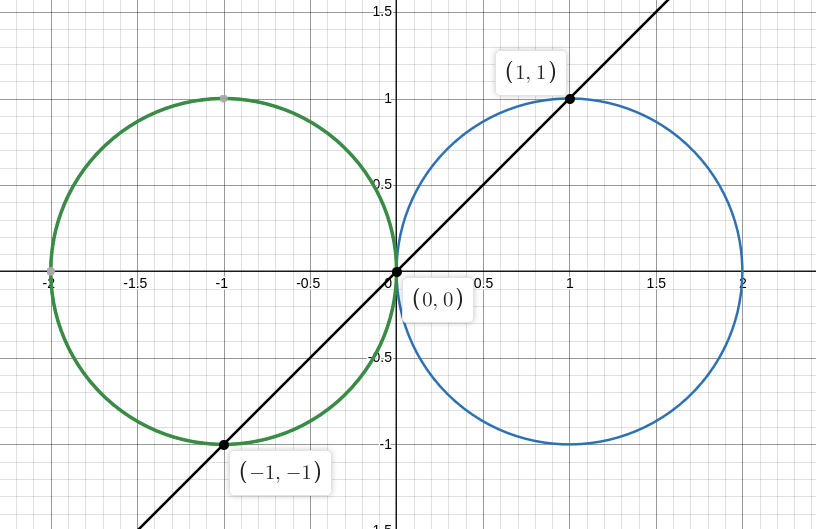
\includegraphics[scale = 0.40]{desmos1.png}
\end{figure}
Because our objective function is linear, the local minimizer and the global minimizer are the same value. We determine that (-1, -1) is both our global and local minimizer.
\break
\break
\textbf{Problem 2.5:} In this exercise we are tasked with providing an example function that nas no global minimizer and no global maximizer. If we take any linear function without constraints we will have no global minimizer or maximizer. The function $f(x) = x_1$ for example.

       
\end{document}
